\section{Arquitectura base (C4)}

La arquitectura se documenta con dos niveles del modelo C4. Los archivos editables de draw.io están en \texttt{docs/diagramas/}.

\subsection{Nivel 1: contexto}

El diagrama de contexto muestra el sistema con sus usuarios (Vicerrectorado, evaluadores, postulantes y administrador) y los sistemas externos con los que se comunica: correo, Supabase Storage, Google Drive, y los proveedores de IA (Groq, Mistral y Hugging Face).

\begin{figure}[p]
  \centering
  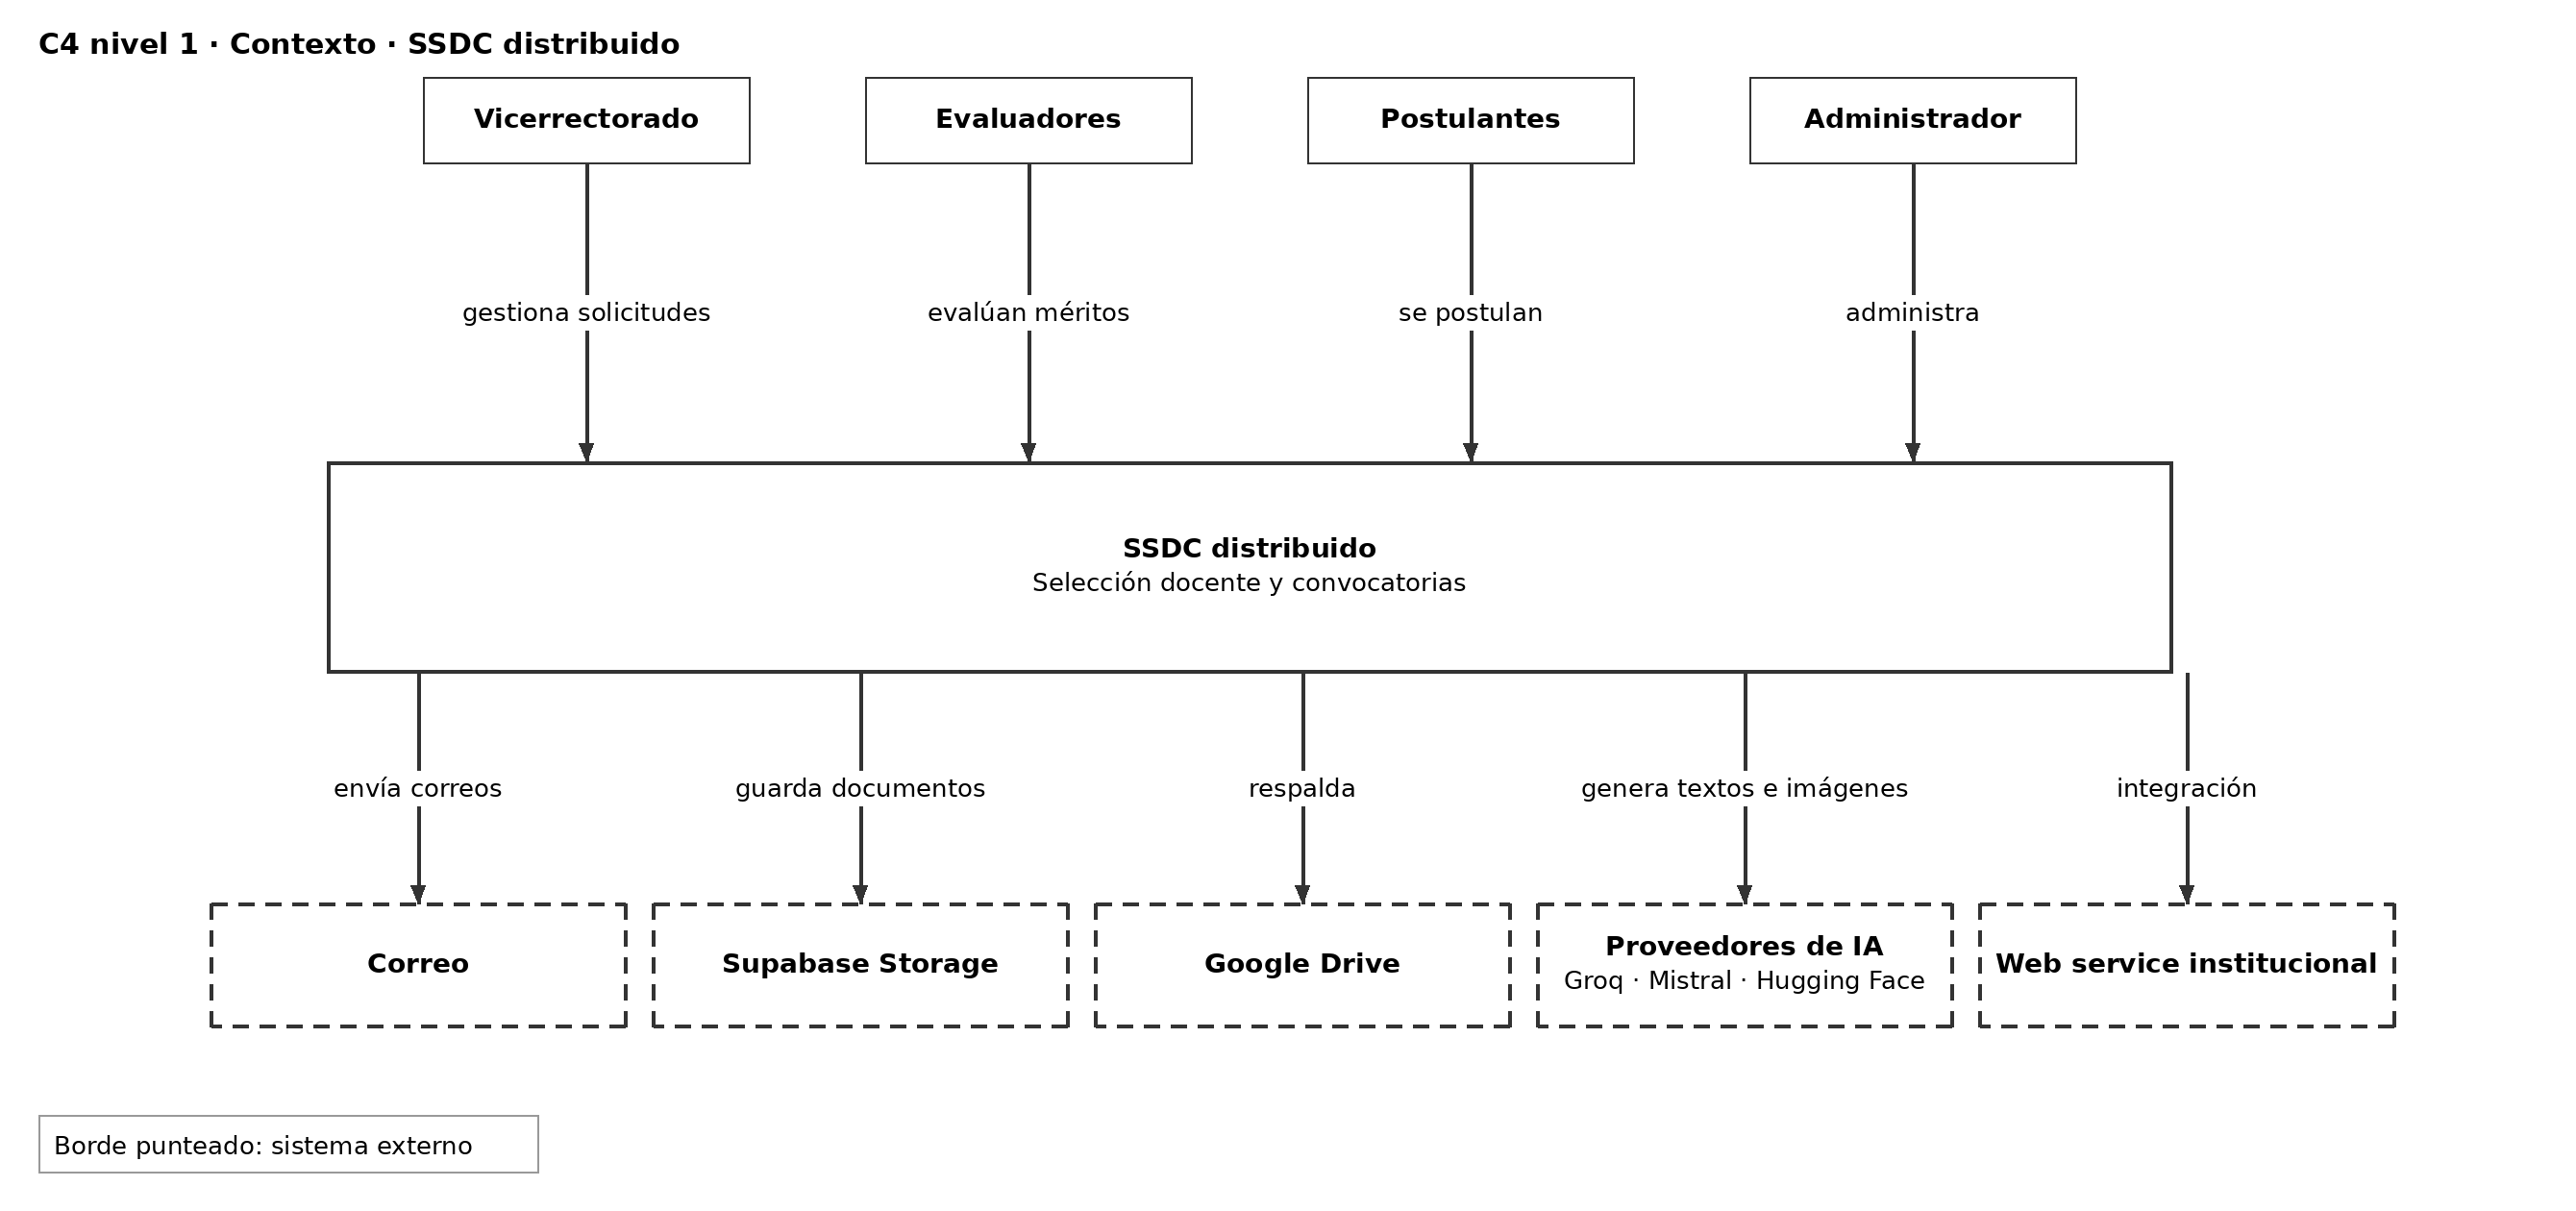
\includegraphics[width=0.93\textheight,angle=90]{c4-nivel1-contexto.png}
  \caption{C4 nivel 1: contexto del SSDC distribuido.}
\end{figure}

\subsection{Nivel 2: contenedores}

El diagrama de contenedores muestra un frontend, un API gateway que valida el token y seis servicios. Cuatro de ellos tienen su propia base PostgreSQL: postulaciones, evaluación, convocatorias y auditoría. \texttt{convocatorias} y \texttt{notificaciones} están implementados en el esqueleto de \texttt{src/} y se comunican por HTTP. Los otros cuatro servicios, el API gateway (que validaría el token) y la cola de mensajes están planeados; el uso de la cola lo define el ADR-002.

\begin{figure}[p]
  \centering
  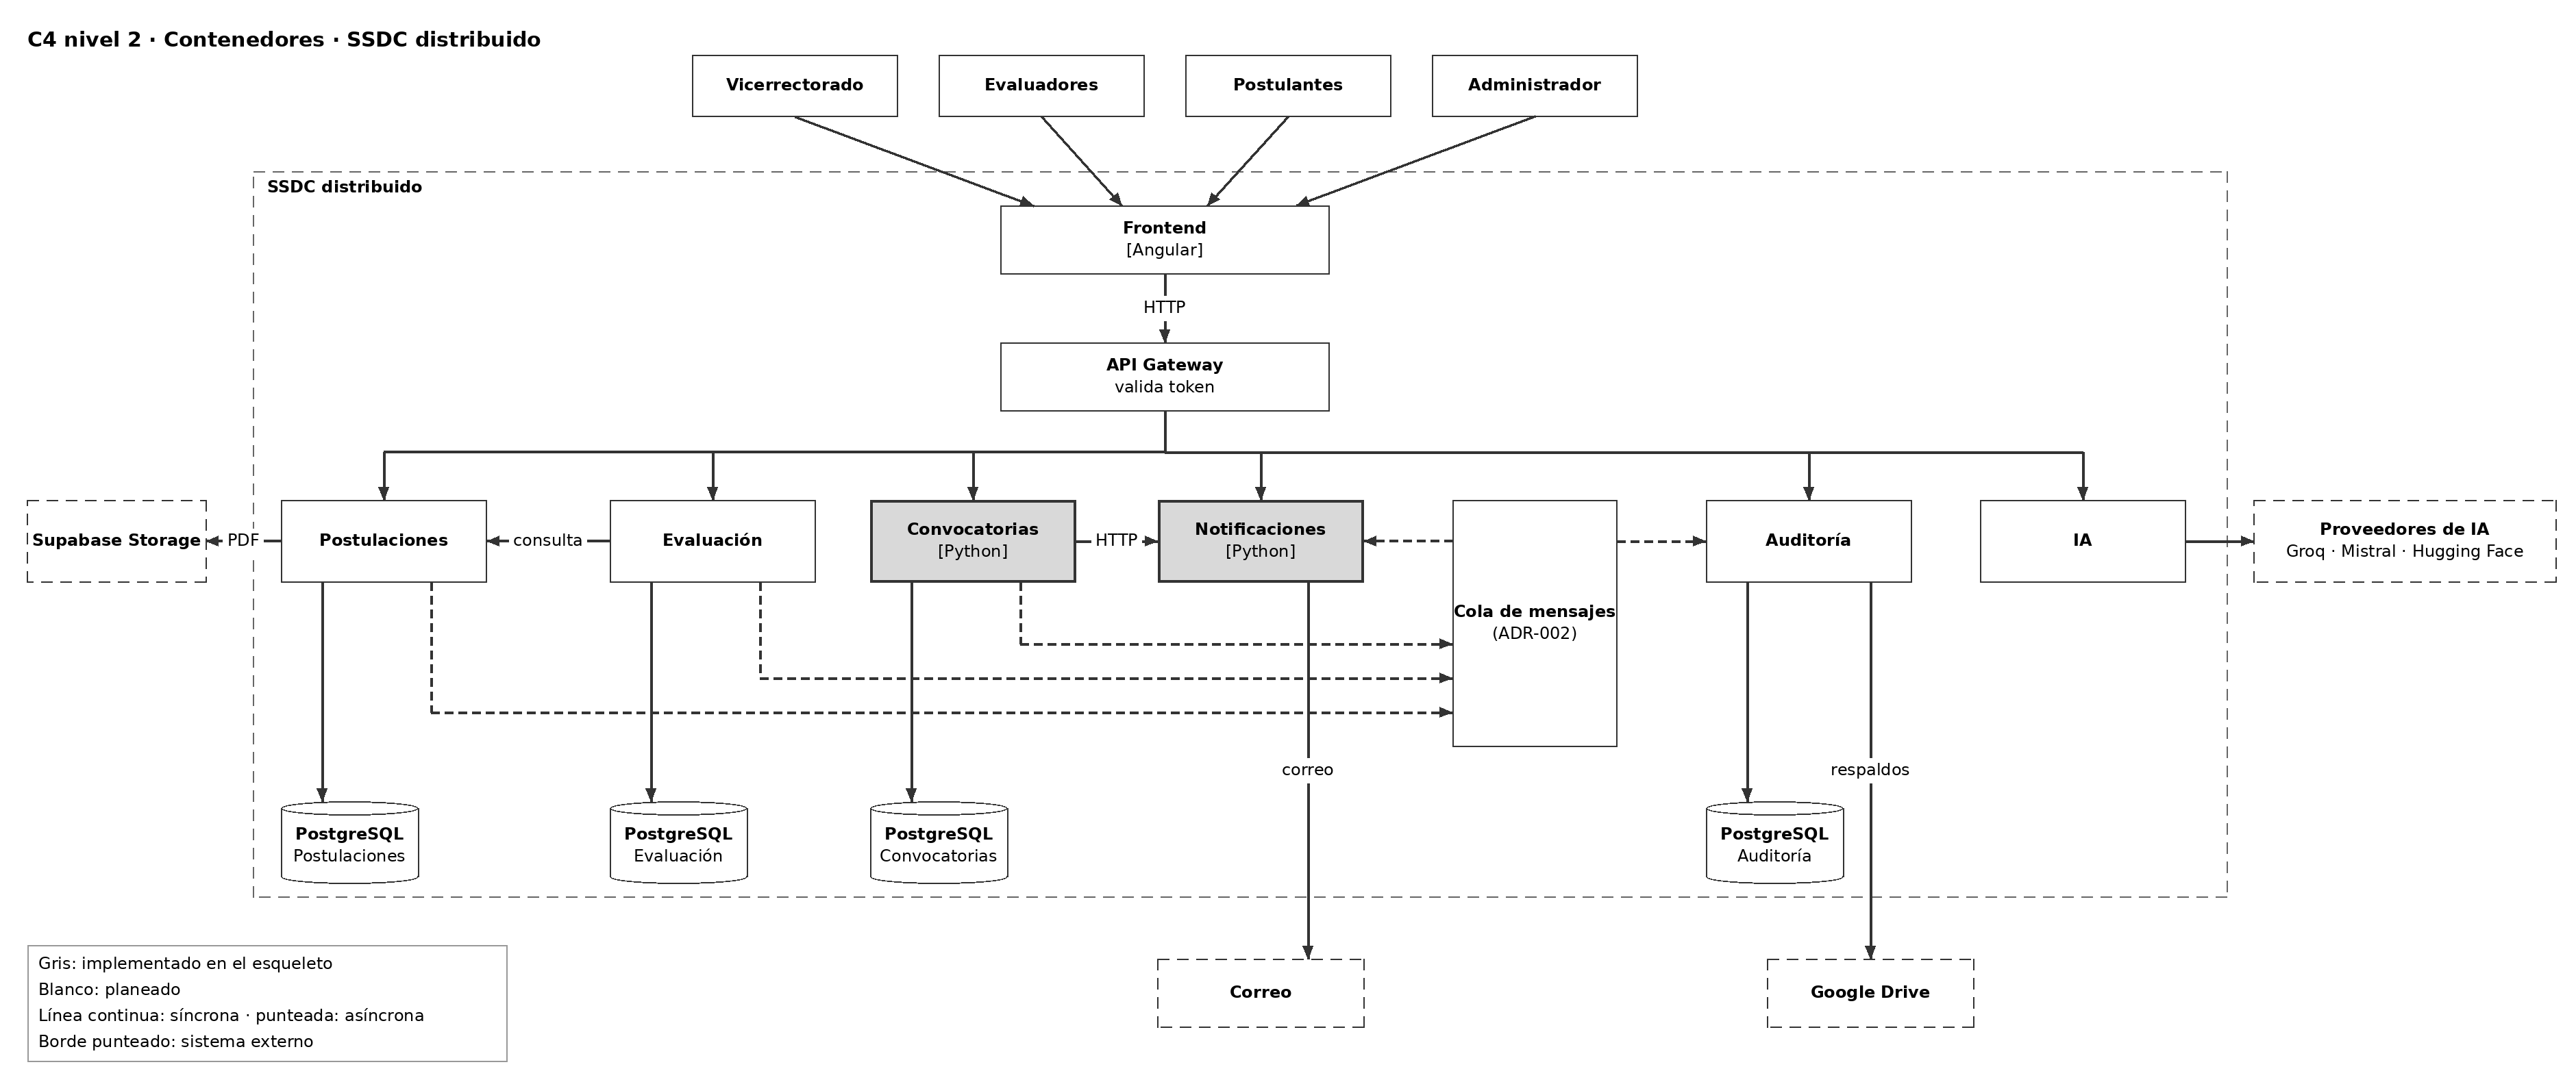
\includegraphics[width=0.93\textheight,angle=90]{c4-nivel2-contenedores.png}
  \caption{C4 nivel 2: contenedores del SSDC distribuido. En gris, los servicios implementados en el esqueleto.}
\end{figure}

\begin{table}[H]
\centering
\small
\caption{Contenedores del sistema}
\begin{tabularx}{\linewidth}{@{}p{3.1cm}p{2.7cm}X@{}}
\toprule
\textbf{Contenedor} & \textbf{Estado} & \textbf{Responsabilidad} \\
\midrule
\texttt{convocatorias} & esqueleto & Lista y publica convocatorias, y al publicar avisa a \texttt{notificaciones} por HTTP. Planeado: solicitudes docentes y creación de convocatorias. \\
\texttt{notificaciones} & esqueleto & Recibe avisos, los guarda en memoria y los lista. Planeado: envío del correo de cambio de estado. \\
\texttt{postulaciones} & planeado & Prepostulación, expediente en PDF (Supabase Storage) y estado de la postulación. \\
\texttt{evaluacion} & planeado & Matriz de méritos, ranking, entrevistas y clases demostrativas. Consulta a \texttt{postulaciones}. \\
\texttt{auditoria} & planeado & Registro de cambios con hash SHA-256 y respaldos hacia Google Drive. \\
\texttt{ia} & planeado & Generación asistida de textos e imágenes con proveedores externos. \\
\bottomrule
\end{tabularx}
\end{table}
